\begin{frame}{Normal mapping}
	\pause
	\begin{columns}
		\begin{column}{0.33\textwidth}
			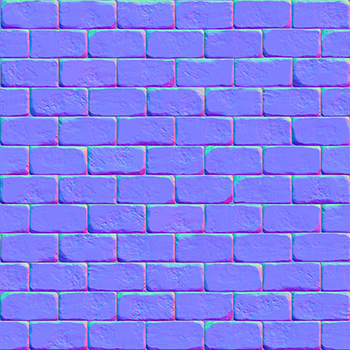
\includegraphics[width=\textwidth]{normal_map}
		\end{column}
		\begin{column}{0.65\textwidth}
			\begin{itemize}
				\item A \textbf{normal map} is a texture which is used to slightly alter the normal
					across a surface
					\begin{itemize}
						\pause\item Each pixel in the normal map represents a 3D vector, with $xyz$ mapped to RGB
					\end{itemize}
			\end{itemize}
		\end{column}
	\end{columns}
	\pause
	\begin{columns}
		\begin{column}{0.33\textwidth}
			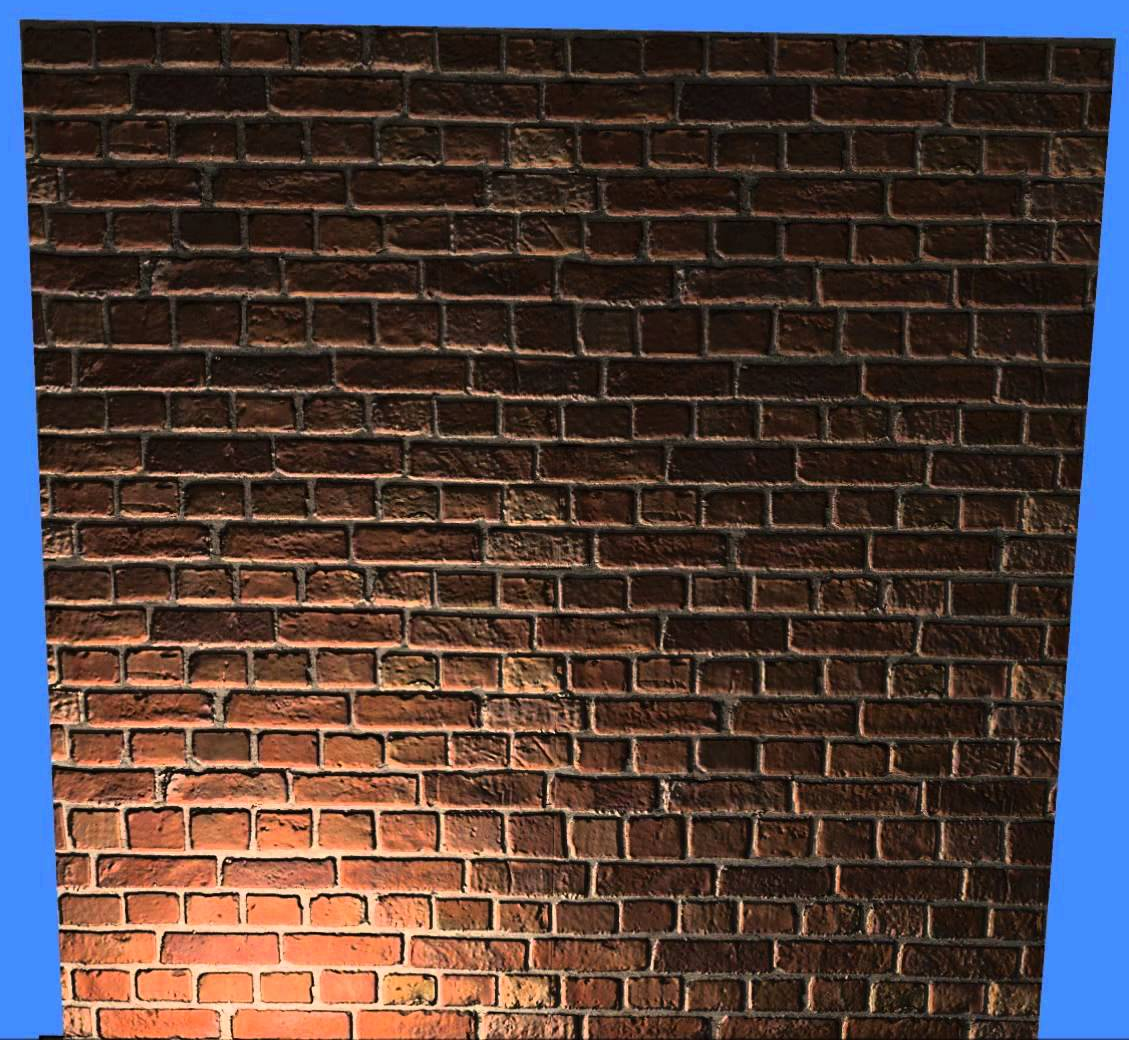
\includegraphics[width=\textwidth]{normal_mapped_wall}
		\end{column}
		\begin{column}{0.65\textwidth}
			\begin{itemize}
				\item Can be used to add detail to flat, low-poly surfaces
				\pause\item Can use textures to change other lighting parameters across a surface,
					e.g.\ \textbf{specular mapping}
			\end{itemize}
		\end{column}
	\end{columns}
\end{frame}